\documentclass[../report.tex]{subfiles}
\begin{document}

\onehalfspacing

\section{System Design}

Verification across the Hardware Firmware boundary requires a system that utilizes both Hardware and Firmware in equal parts to achieve a single goal.
A secure bootloader is a program that ensures only encrypted and authenticated software is loaded onto a platform~\cite{secure-bootloader}.
In order for a bootloader to be secure it must run before any other code is executed on the platform.
Because of this, the bootloader is responsible for doing all system initialization, including hardware initialization of modules.
The bootloading process must also complete before any of the other platform code is run, meaning that program speed is important. 
The cryptographic functions of hashing and signing the authenticated software are computationally expensive and are therefore offloaded to hardware accelerators. 
All of these factors make secure boot ideal for formal verification techniques.

Verified Boot is an implementation of secure boot that has been designed by Google to run on their Chromebook laptops.
Verified Boot is the bootloader to the Chrome Operating System and verifies that all system code has been signed by Google.
Google has released both Verified Boot and Chrome OS as Open Source software, making this a viable candidate for formal verification.
While the specific hardware in each laptop is still closed source, Google has documents for extending their Verified Boot program and outlines the minimum
number of hardware modules required for security.

The hardware modules can be broken into two groups, secure storage and hardware accelerator.
Under secure storage there is an Flash memory module that provides non-volatile storage, and a Trusted Platform Module (TPM) that provides non-volatile storage that can be locked until the next boot.
Under hardware accelerators there are the cryptographic functions implementing Secure Hash Algorithm (SHA) and RSA encryption. 
The CPU accesses the hardware modules through different protocols as seen in Figure. %TODO
These interaction methods can be abstracted to Memory Mapped I/O without losing security information.

\subsection{Hardware}

\subsubsection{Flash Memory}

Each Chrome book comes with 8 Mbs of non-volatile Flash memory~\cite{fw-summit}.
The memory is organized according to Figure~\ref{fig:fmap}. 
The Flash memory is connected to the CPU by the Serial Peripheral Interface (SPI).
The SPI driver handles the protocol and provides an interface for reading multiple bytes of of memory at once.
% TODO: check if there is some sort of mass info transfer, this seems really slow.
The important feature of the Flash Memory is it's hardware protected Read-Only (RO) section of memory.
The RO section is enforced by the placement of a physical screw known as the Write Protect (WP) Screw.
If the WP Screw remains in the laptop, all writes to the RO section will fail.
If the screw is removed, all of Google's security claims can be violated. 
Google is aware of this and considers the warranty of the laptop to be voided if the screw is removed.

The Read-Only memory is flashed into the laptop when the Chromebook is being built in the factory, before the Read-Only screw is added to the casing. 
The Reset Vector of the CPU points to the Read-Only flash memory, and the code located in the RO section provides information to verify the rest of the system.
In this way the RO Flash acts as the ``Root of Trust'' for the system.
In security terms, the Verified Boot process should be secure as long as the Root of Trust holds.
Inversely, if someone removes the WP screw, none of the Verified Boot security properties will hold.

\begin{figure}
  \centering
  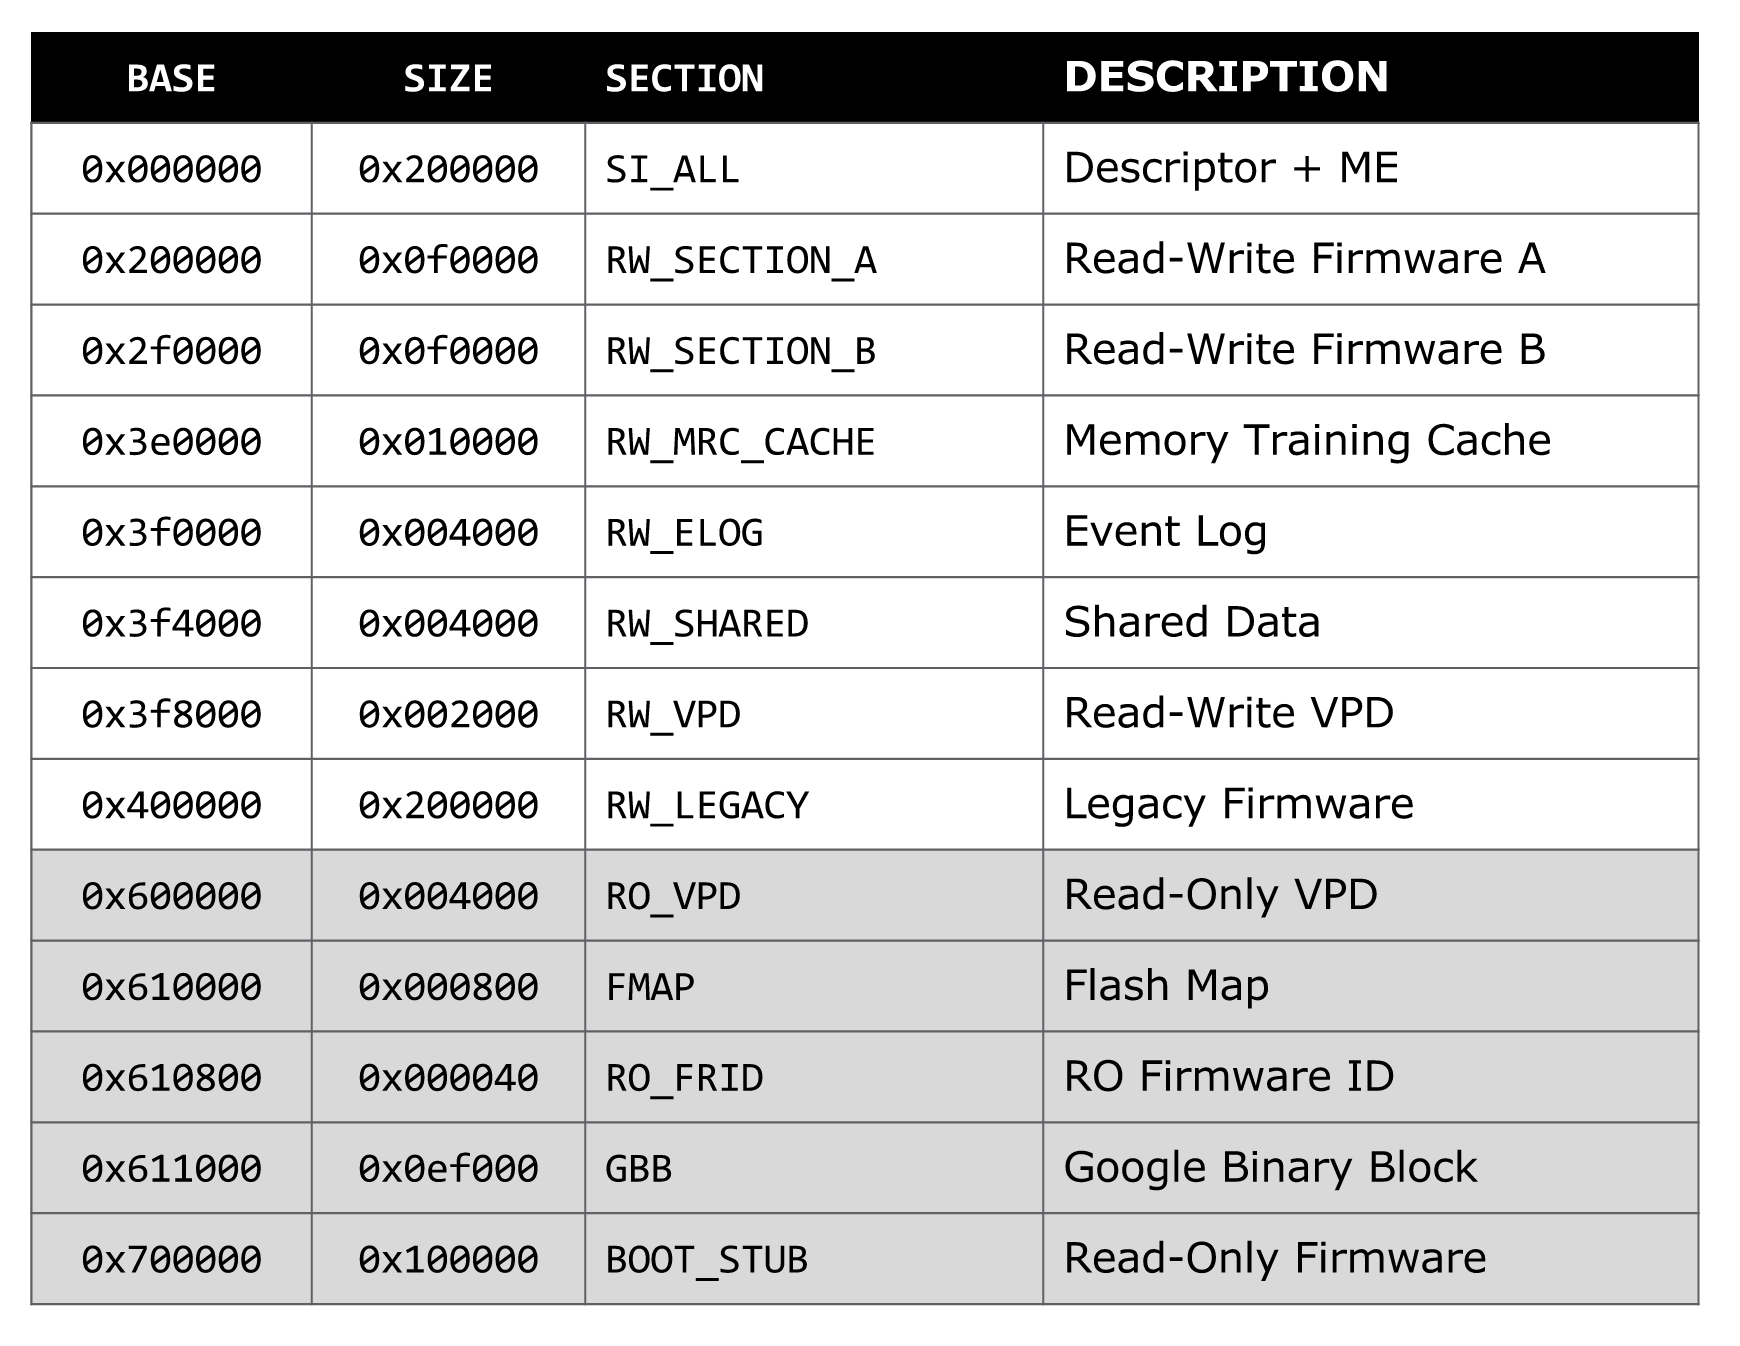
\includegraphics[width=0.8\linewidth]{fmap_locs.png}
  \caption{The Flash Map for Chrome OS's SPI Flash. The gray sections have been marked as Read Only~cite\cite{fw-summit}}
  \label{fig:fmap}
\end{figure}

The organization of the Flash Memory can be seen in Figure~\ref{fig:fmap}.
This map of Flash memory is referred to as the ``fmap'' and it is stored in Flash as can be seen in the figure.
The gray sections of the figure are the Read Only sections and provide the Root of Trust of the boot system as discussed previously.

\subsubsection{TPM}

The Trusted Platform Module or TPM is a generic name for any secure cryptoprocessor that conforms to the standards written by the Trusted Computing Group (TCG). %TODO cite
Although Google has released Chromebooks with both 1.2 and 2.0 TPMs, for the scope of this project we will be looking at the TPM 1.2 specification.

The TPM allows for secure access of non-volatile store, with permissions that can be permanently set until the platform is powered off.
The TPM can also create and store RSA keys as well as perform RSA encryption and decryption. 
The TPM is communicated with by sending binary commands and data as outlined by the TCG. %TODO cite


% \subsubsection{External Controller}

\subsubsection{SHA}
\subsubsection{RSA}

\end{document}
